\cleardoublepage

\chapter{Résultats - Discussions}

%%%%%%%%%%%%%%%%%%%%%%%%%%%%%%%%%%%%%%%%%%%%%%%%%%%%%%%%%%%%%%%%%%%%%%%%%%%
%%%%%%%%%%%%%%%%%%%%%%%%%%%%%%%%%%%%%%%%%%%%%%%%%%%%%%%%%%%%%%%%%%%%%%%%%%%
%%%%%%%%%%%%%%%%%%%%%%%%%%%%%%%%%%%%%%%%%%%%%%%%%%%%%%%%%%%%%%%%%%%%%%%%%%%
%%%%%%%%%%%%%%%%%%%%%%%%%%%%%%%%%%%%%%%%%%%%%%%%%%%%%%%%%%%%%%%%%%%%%%%%%%%
%%%%%%%%%%%%%%%%%%%%%%%%%%%%%%%%%%%%%%%%%%%%%%%%%%%%%%%%%%%%%%%%%%%%%%%%%%%

\section{Interface graphique utilisateur}

J'ai été libre de programmer la première version de l'interface graphique, comportant les fonctionnalités demandées par le client. Ce dernier a participé à sa réalisation en effectuant diverses critiques et réagencements des éléments afin d'optimiser l'ergonomie de l'application.

Je présenterai dans cette section la structure de l'affichage et les différents types d'écran.

%%%%%%%%%%%%%%%%%%%%%%%%%%%%%%%%%%%%%%%%%%%%%%%%%%%%%%%%%%%%%%%%%%%%%%%%%%%
%%%%%%%%%%%%%%%%%%%%%%%%%%%%%%%%%%%%%%%%%%%%%%%%%%%%%%%%%%%%%%%%%%%%%%%%%%%
%%%%%%%%%%%%%%%%%%%%%%%%%%%%%%%%%%%%%%%%%%%%%%%%%%%%%%%%%%%%%%%%%%%%%%%%%%%

\subsection{Structure}

%%%%%%%%%%%%%%%%%%%%%%%%%%%%%%%%%%%%%%%%%%%%%%%%%%%%%%%%%%%%%%%%%%%%%%%%%%%

\subsubsection{Barre supérieure}

La partie supérieure de l'écran possèdes deux fonctions. La première est l'affichage des détails de l'application : logo, nom de l'application, version. La seconde est liée au compte de l'utilisateur : lien permettant de changer d'utilisateur, de déconnexion, et permettant de quitter l'application.

%%%%%%%%%%%%%%%%%%%%%%%%%%%%%%%%%%%%%%%%%%%%%%%%%%%%%%%%%%%%%%%%%%%%%%%%%%%

\subsubsection{Menu latéral}

Une barre latéral située sur la partie gauche propose un \textit{menu}. Chaque ligne de ce menu correspond à un module de l'application. La figure \ref{menu} est une capture d'écran du menu, montrant les différents menus, et donc modules, de l'application.

De plus, un sous-menu de second niveau apparait lorsque l'on sélectionne un menu. Il s'agit de chacun des écrans principaux du module correspondant. Par exemple, le menu "Accès" possède quatre sous-menus correspondants à quatre fonctionnalités, comme le montre la figure \ref{menu_administration}.

%\begin{figure}[!h]
%	\center
%	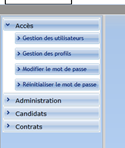
\includegraphics[width=2cm]{img/appli/menu.png}
%	\caption{Menu latéral gauche}
%	\label{menu}
%\end{figure}

%%%%%%%%%%%%%%%%%%%%%%%%%%%%%%%%%%%%%%%%%%%%%%%%%%%%%%%%%%%%%%%%%%%%%%%%%%%
%%%%%%%%%%%%%%%%%%%%%%%%%%%%%%%%%%%%%%%%%%%%%%%%%%%%%%%%%%%%%%%%%%%%%%%%%%%
%%%%%%%%%%%%%%%%%%%%%%%%%%%%%%%%%%%%%%%%%%%%%%%%%%%%%%%%%%%%%%%%%%%%%%%%%%%

\subsection{Les types d'écran}

Les écrans peuvent peuvent être de plusieurs types.

Un écran d'affichage de données comporte un tableau permettant d'afficher une liste de valeurs. Il y a une zone de recherche permettant de filtrer les données. De plus, des boutons situés en bas de l'écran permettent d'effectuer des actions sur le ou les élément(s) sélectionné(s) : affichage des détails, modification, suppression, \ldots

L'affichage, la modification ou la création d'un élément est une fenêtre s'affichant par dessus l'écran actuel sous la forme d'un pop-up. Lorsqu'il s'agit d'une édition, les éléments sont des "zones de texte" ou des "listes déroulantes", sinon ce sont simplement des "labels".

Des écrans de "paramétrage" permettent la gestion des tables "statiques". Ce sont les valeurs des différentes listes déroulantes que l'on peut trouver dans les écrans de saisie. Il est ainsi possible d'administrer ces listes en supprimant certaines entrées ou en créant de nouvelles.

%%%%%%%%%%%%%%%%%%%%%%%%%%%%%%%%%%%%%%%%%%%%%%%%%%%%%%%%%%%%%%%%%%%%%%%%%%%
%%%%%%%%%%%%%%%%%%%%%%%%%%%%%%%%%%%%%%%%%%%%%%%%%%%%%%%%%%%%%%%%%%%%%%%%%%%
%%%%%%%%%%%%%%%%%%%%%%%%%%%%%%%%%%%%%%%%%%%%%%%%%%%%%%%%%%%%%%%%%%%%%%%%%%%
%%%%%%%%%%%%%%%%%%%%%%%%%%%%%%%%%%%%%%%%%%%%%%%%%%%%%%%%%%%%%%%%%%%%%%%%%%%
%%%%%%%%%%%%%%%%%%%%%%%%%%%%%%%%%%%%%%%%%%%%%%%%%%%%%%%%%%%%%%%%%%%%%%%%%%%

\section{Base de données}

Le modèle de données actuel satisfait bien le besoin du client. Il modélise correctement les différentes données à enregistrer, avec les contraintes et dépendances imposées.

Cependant il reste quelques améliorations possibles. En effet, le client a tendance à ajouter, modifier ou supprimer certaines spécifications au court du projet, imposant des changes plus ou moins importants dans le modèle. Ces changements impactent aussi les différentes couches de l'application, du mapping à l'interface graphique, ce qui peut faire perdre un temps important en fin de projet. Ainsi les modifications "non bloquantes" n'ont pas été apportées et le seront lors du lot 2.





~~\\-------------

TODO: DAPE, DUE